% --------------------------------------------------------------------------
% Template for Project Course paper; to be used with:
%          ProjectCourse21.sty  - Project Course 2021 LaTeX style file, and
%
% --------------------------------------------------------------------------

\documentclass{article}
\usepackage{MAECapstoneCourse,amsmath,graphicx,url,times}
\usepackage{color}
\usepackage[utf8]{inputenc}
\pagenumbering{arabic}

% Example definitions.
% --------------------
\def\defeqn{\stackrel{\triangle}{=}}
\newcommand{\symvec}[1]{{\mbox{\boldmath $#1$}}}
\newcommand{\symmat}[1]{{\mbox{\boldmath $#1$}}}

% Title.
% --------------------
\title{Sound Event Classification}

% PUT NAMES IN ALPHABETIC ORDER (consider surname first)
\name{Chiara Auriemma, Francesca Benesso, Anna Fusari, Filippo Marri}
\address{Dipartimento di Elettronica, Informazione e Bioingegneria (DEIB), Politecnico di Milano\\
Piazza Leonardo Da Vinci 32, 20122 Milano, Italy\\   
\tt{[chiara.auriemma,francesca1.benesso]@mail.polimi.it}\\
\tt{[anna.fusari,filippo.marri]@mail.polimi.it}
}

\begin{document}

\ninept
\maketitle

\begin{sloppy}

\begin{abstract}
  Sound Event Classification (SEC) has become an important task in the field of
  audio processing, with applications ranging from environmental monitoring to
  human-computer interaction. Aim of this project is to develop a sound event classification system
  based on a Convolutional Neural Network (CNN) architecture training it on the ESC-50 dataset.
  At the end, the performances of the model are compared with some state-of-the-art models (QUALE?).
  [Da finire, deve essere una sorta di riassunto del progetto, con le tecniche utilizzate e i risultati ottenuti].
\end{abstract}

\begin{keywords}
Sound Event Classification, Convolutional Neural Network, ESC-50 dataset, performance limitations
\end{keywords}

\section{Introduction}
\label{sec:intro}

\subsection{Background}
\label{sec:background}
Sound Event Classification (SEC) is a task that involves classification of
specific sound events within an audio signal. This task has gained significant attention in recent years
due to its wide range of applications, including environmental monitoring \cite{birdsCNN2017}, human-computer interaction \cite{emotionRecognition2021},
and multimedia content analysis \cite{kumar2016weaklysupervisedscalableaudio}.
The goal of SEC is to accurately classify sound events in real-time or from pre-recorded audio data.
The process of SEC typically involves several steps, including feature extraction, model training, and evaluation \cite{ReviewSoundEvent2025}.

Commonly used features include Mel-frequency cepstral coefficients (MFCCs), log-spectrograms, and log-mel spectrograms.
Model training involves using labeled audio data to train a machine learning model to classify sound events.
Various machine learning algorithms can be used for SEC, including support vector machines (SVMs), decision trees, and deep
learning models such as convolutional neural networks (CNNs) and recurrent neural networks (RNNs) \cite{DescriptiveESC2022}.
The choice of algorithm depends on the complexity of the task and the available data.

Evaluation of the SEC system is typically done using standard metrics such as accuracy, precision, recall, and F1-score.

\subsection{Literature review for project development}
\label{sec:literature_review_project_development}
One of the first attempts in SEC was made by Piczak \cite{Piczak2015environmental} in 2015, in which the sound is split in several segments
and each segment is processed individually using a Convolutional Neural Network (CNN). At the end a series of Dense Layer is used to classify the segments.
Final predictions for a sound are generated using either a majority-voting scheme or by taking into account the
probabilities predicted for each segment.



\section{Methodology}
\label{sec:methodology}
As a baseline of this project we chose a simple 2D Convolutional Neural Network (CNN) architecture based on the CONV2D model of laboratory number 4.
We chose a 2D Convolutional network since we have, as input, a log mel-spectrogram. In turn, this kind of input has been chosen in order to feed the network with
temporal-frequency correalated data, approach widely followed in the literature. However, the results obtained with this architecture were not satisfactory,
so we decided to improve the model by adding some layers and using a more complex architecture. After several attempts with Recurrent Convolutional Neural Networks (CRNN),
we opted for a multi-branch convolutional neural network (MBCNN) architecture inspired by the work of Enes Furkan Örnek \cite{audio_classification_esc50, latifi2025classificationheartsoundsusing}.

\subsection{Feature extraction}
\label{sec:feature_extraction}
As hinted before, the neural network is fed with a log mel-spectrogram, computed by a specific function that takes as input
the signal preserving its original sample rate. The parameters are the following:
\begin{itemize}
    \item \textbf{N fft}: 1024 samples
    \item \textbf{Hop size}: 512 samples
    \item \textbf{Number of mel bands}: 128 (predefined parameter)
\end{itemize}
The output is a 2D array of shape (128, 1723) representing how energy in different Mel frequency bands evolves over time.

\subsection{Model description}
\label{sec:model_description}
The model code can be found at the following link:

\url{https://github.com/ChiaraAuriemma/Sound-Event-Classification}.


Our implementation utilizes a bi-dimensional Convolutional Neural Network (CNN)
with four parallel branches, each extracting different levels of information from the
input data using specifically calibrated kernel sizes. 
We highlight that our model is working in a peculiar way with the 2D layers since one dimension is, layer-by-layer, alternatively
imposed equal to 1. With this method, each branch alternates between horizontal and vertical filter orientations,
enabling efficient extraction of localized patterns across both time and frequency domains.
The net is built following a cellular approach. Each cell is composed by a Conv2D layer followed by batch normalization and
ReLU activationin in order to ensure training stability and non-linearity as its shown in figure~\ref{fig:simple_cell}.
[Commento: after each Conv2D layer, we apply batch normalization and ReLU activationin order to ensure training stability and non-linearity.]
\begin{figure}[ht]
  \centering
  \centerline{\includegraphics[width=\columnwidth]{simple_cell.png}}
  \caption{Structure of a cell of the architecture.}
  \label{fig:simple_cell}
\end{figure}

After processing through these branches, the outputs are merged via element-wise addition, followed by additional convolutional
layers with larger filter depths to further abstract the combined feature maps. 
A global average pooling layer condenses the
spatial information, and the network concludes with a dense softmax layer that outputs class probabilities over 50 categories.
The entire architecture is depicted in Figure~\ref{fig:Entire_architecture}.
\begin{figure}[ht]
  \centering
  \centerline{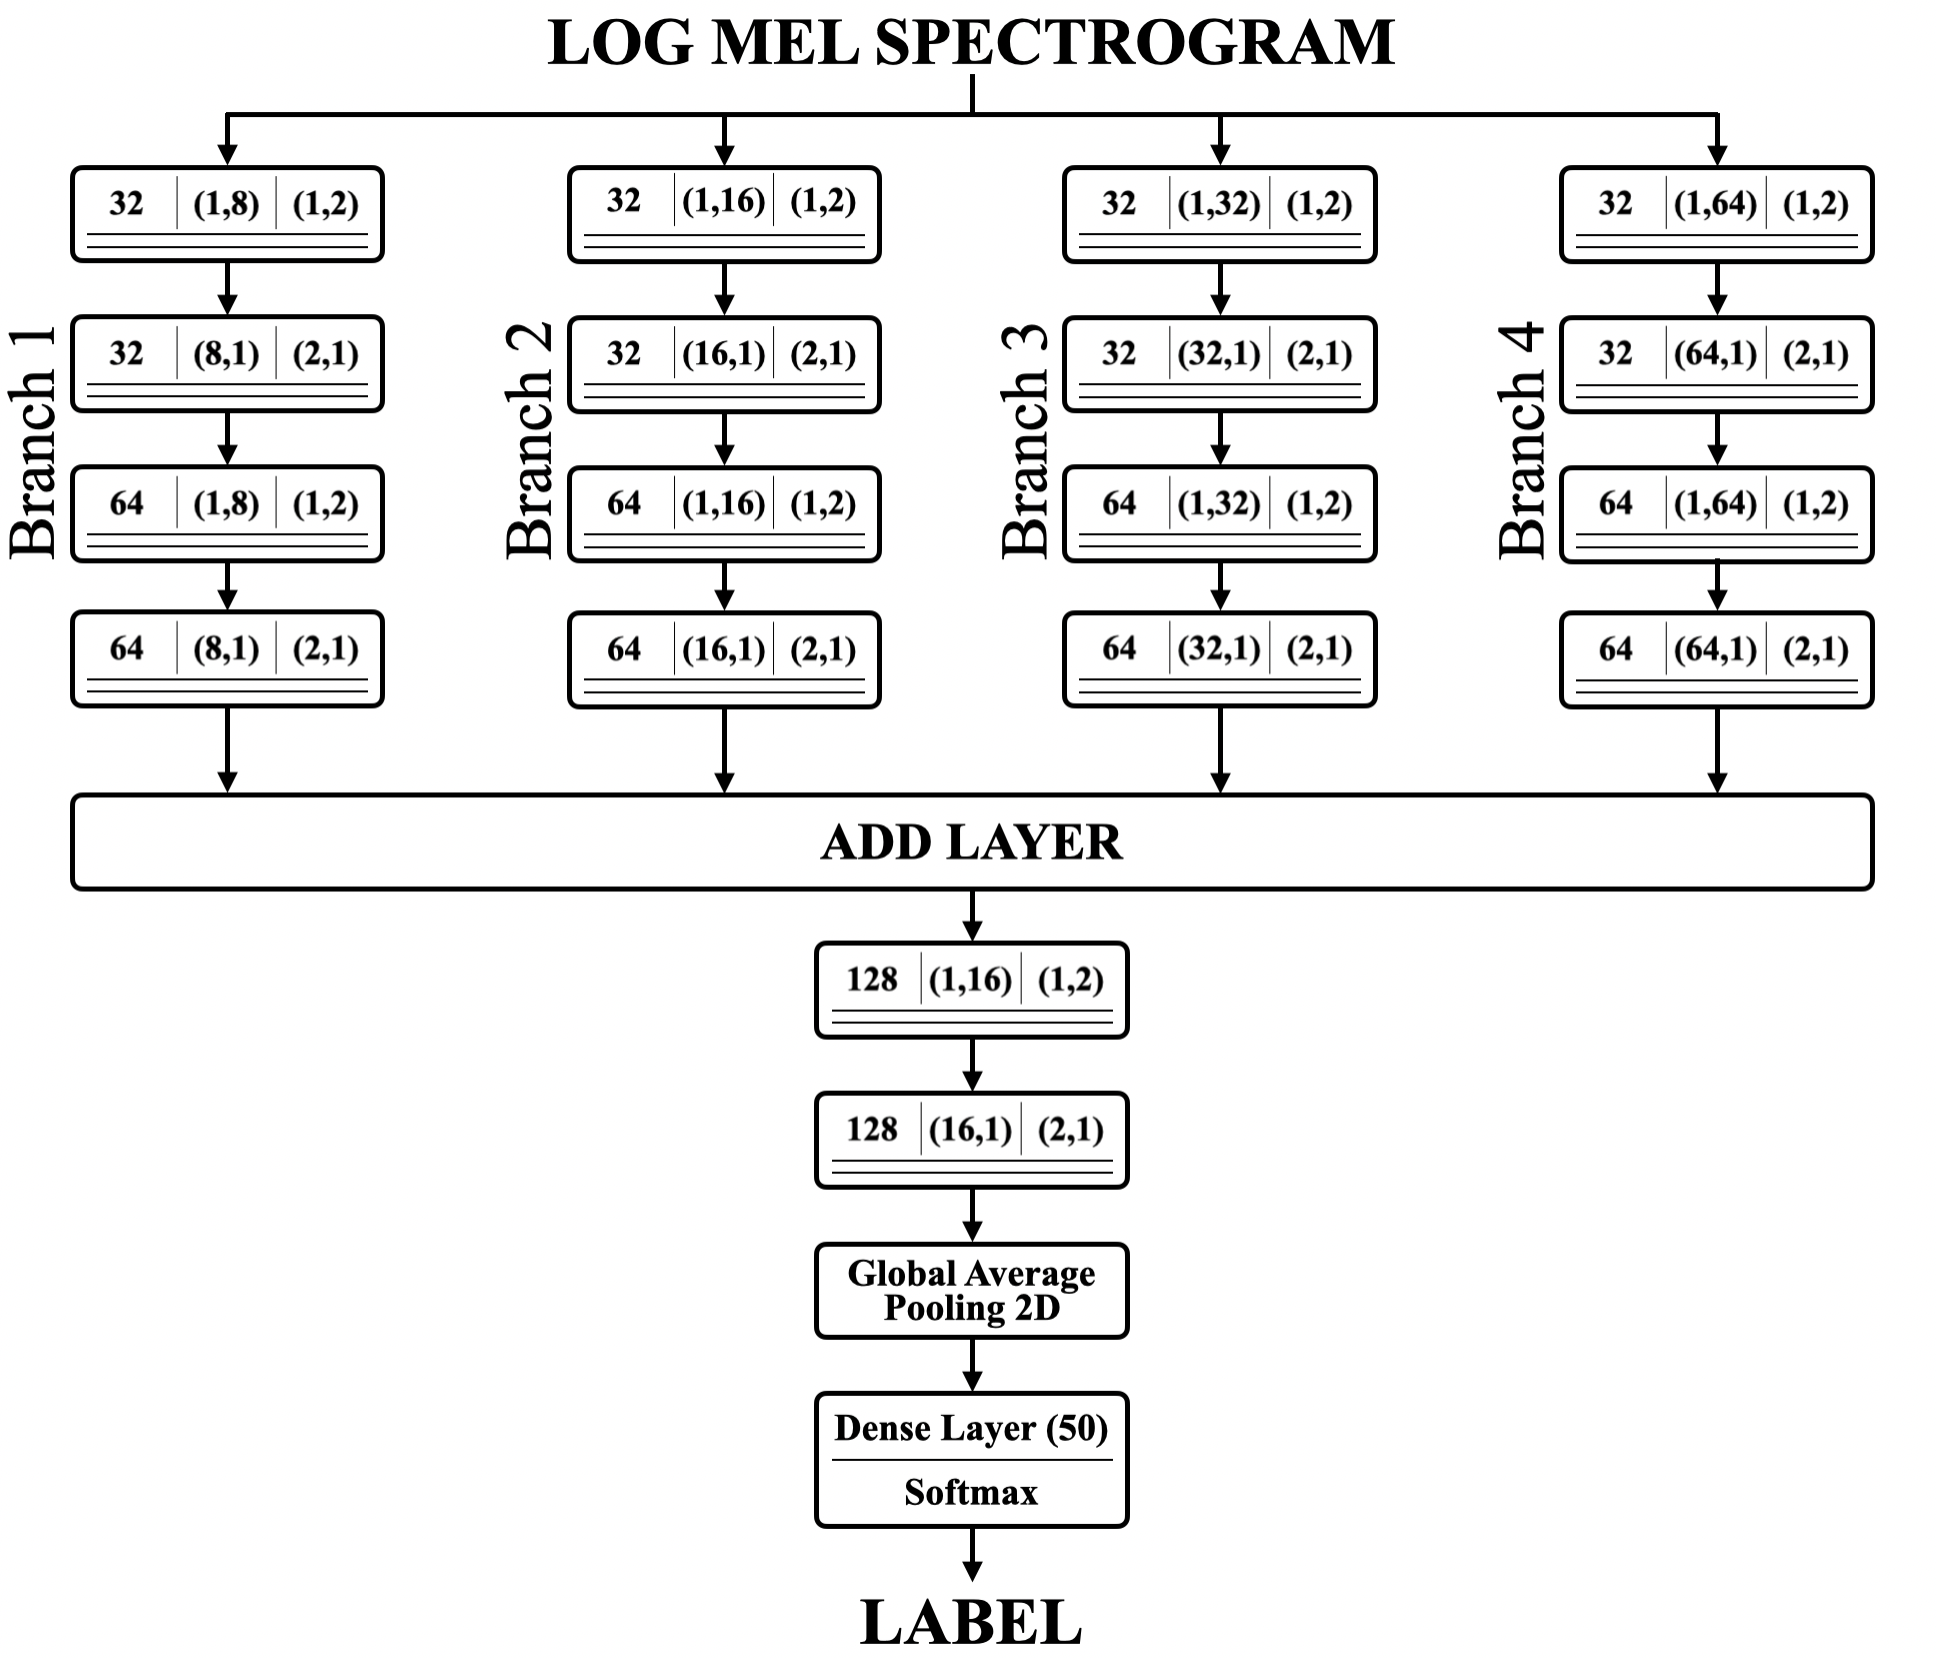
\includegraphics[width=\columnwidth]{Entire_architecture.png}}
  \caption{Architecture of the multi-branch convolutional neural network.}
  \label{fig:Entire_architecture}
\end{figure}

The model is optimized using the Adam optimizer with AMSGrad and learning rate equal to 0.00005, and trained using sparse categorical cross-entropy loss.

The theoretical justification for our filter size selection derives from signal processing
principles in audio analysis. Smaller filters (1×8) effectively capture localized
patterns and high-frequency components, while larger filters (1×64) extract broader
patterns and low-frequency information.

Not only mathematical reasons justify our approach, but also biological ones. In facts, the human auditory system employs a wave bank filter mechanism
to capture specific frequency components in audio signals, with different regions of the
basilar membrane responding to distinct frequency ranges. By incorporating parallel
branches with carefully selected filter sizes, the network similarly detects patterns within specific frequency ranges, enabling multiscale
feature representation.
\section{Evaluation}
\label{sec:evaluation}

\subsection{Dataset analysis and preprocessing}
\label{sec:format}

The dataset used for this project is the well-known ESC-50 dataset \cite{piczak2015dataset}, which contains
2000 labeled isolated eviromental sound events from 50 different classes, with each class containing 40 samples.
Each sound of the dataset is a mono recording available in WAV format (Ogg Vorbis
compress at 192 kbit/s) with a sample rate of 44.1 kHz and a bit depth of 16 bits.
Clips in this dataset have been manually extracted from public field recordings gathered
by the Freesound project \cite{fonseca2020fsd50k}. The resulting dataset is available under a Creative Com-
mons non-commercial license through the Harvard Dataverse project \cite{piczak2015dataset}.

\begin{figure}[ht]
  \centering
  \centerline{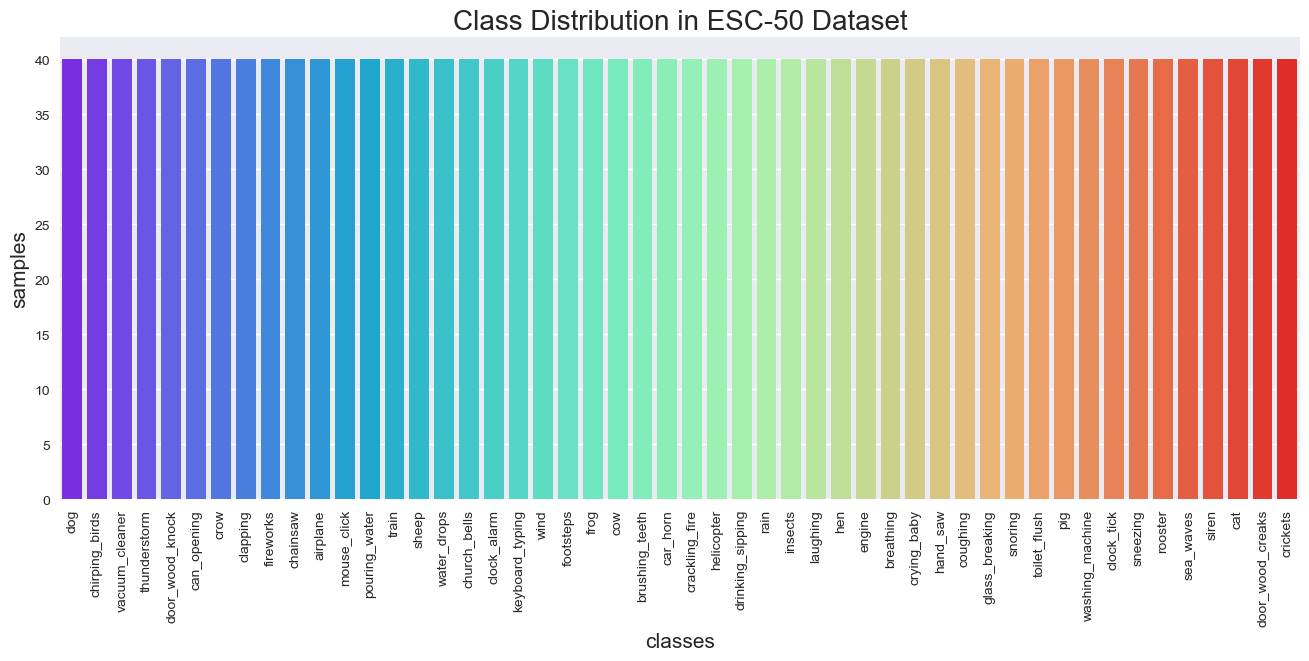
\includegraphics[width=\columnwidth]{balanced_dataset.png}}
  \caption{Graphical demontration of the balance of the dataset used.}
  \label{fig:balanced_dataset}
\end{figure}

According to the analysis that will be done on the results inspired by \textit{Attention based Convolutional Recurrent Neural Network for Environmental Sound Classification} \cite{zhang2019attentionbasedconvolutionalrecurrent}, the type of soound events in the dataset can be divided into three main categories:
\begin{itemize}
    \item \textbf{Transient sounds}: this category includes sounds that have a short duration and are characterized by a sudden onset, such as the one of a glass breaking, a thunderstorm, or a firework.
    \item \textbf{Continous sounds}: this category includes sounds that have a longer duration and are characterized by a continuous or sustained sound, such as the one a vacuum cleaner, a car engine running, or pouring water.
    \item \textbf{Intermittent sounds}: this category includes sounds that have a periodic or irregular pattern, such as the one a dog barking, a bird chirping, or a man coughing.
\end{itemize}
Some examples are reported in Fig.~\ref{fig:power_spectrograms_3_sounds}, where we can see the power spectrogram of a transient sound (glass breaking), a continuous sound (vacuum cleaner), and an intermittent sound (dog barking).

\begin{figure}[ht]
  \centering
  \centerline{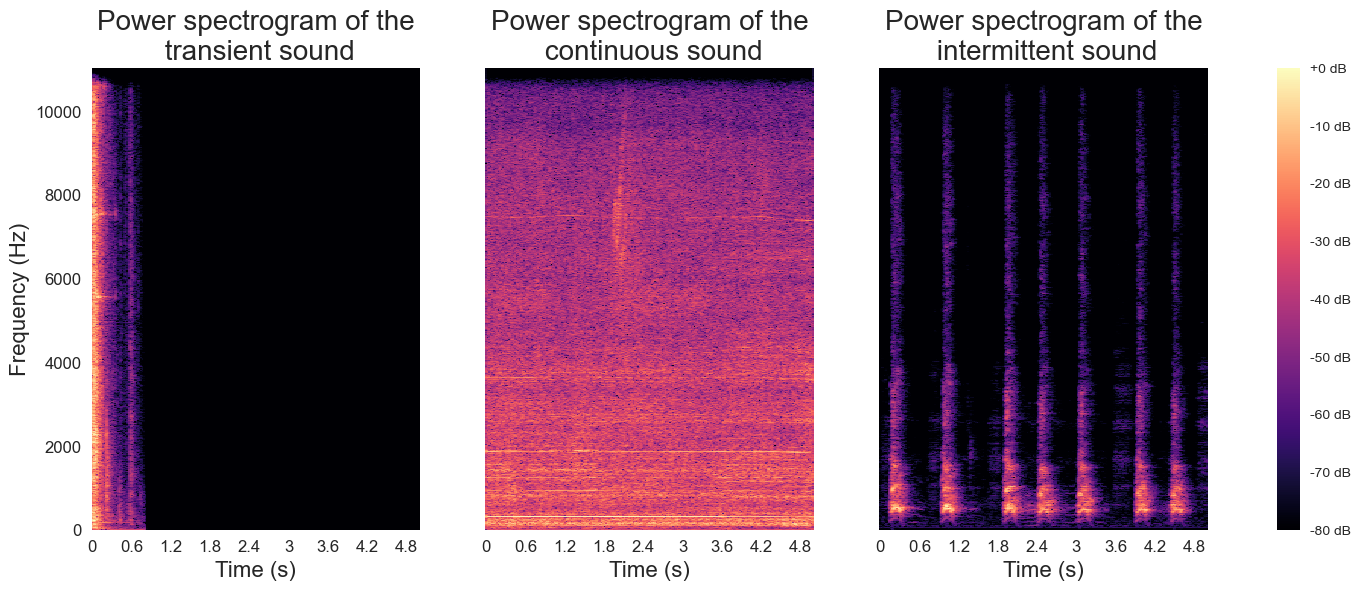
\includegraphics[width=\columnwidth]{Three_types_of_sound.png}}
  \caption{Power spectrogram of a transient, a continous and an intermittent sound.}
  \label{fig:power_spectrograms_3_sounds}
\end{figure}

According to what is reported on the paper in which the ESC-50 dataset is presented \cite{piczak2015dataset}, we higlight how some sounds are more difficult to classify than others,
such as the sounds of a washing machine, an helicopter, or an engine due to their similar spectrograms. If we look to Fig.~\ref{fig:Ambiguous_sounds}, we can see how the three spectrograms
are extremely similar.

\begin{figure}[ht]
  \centering
  \centerline{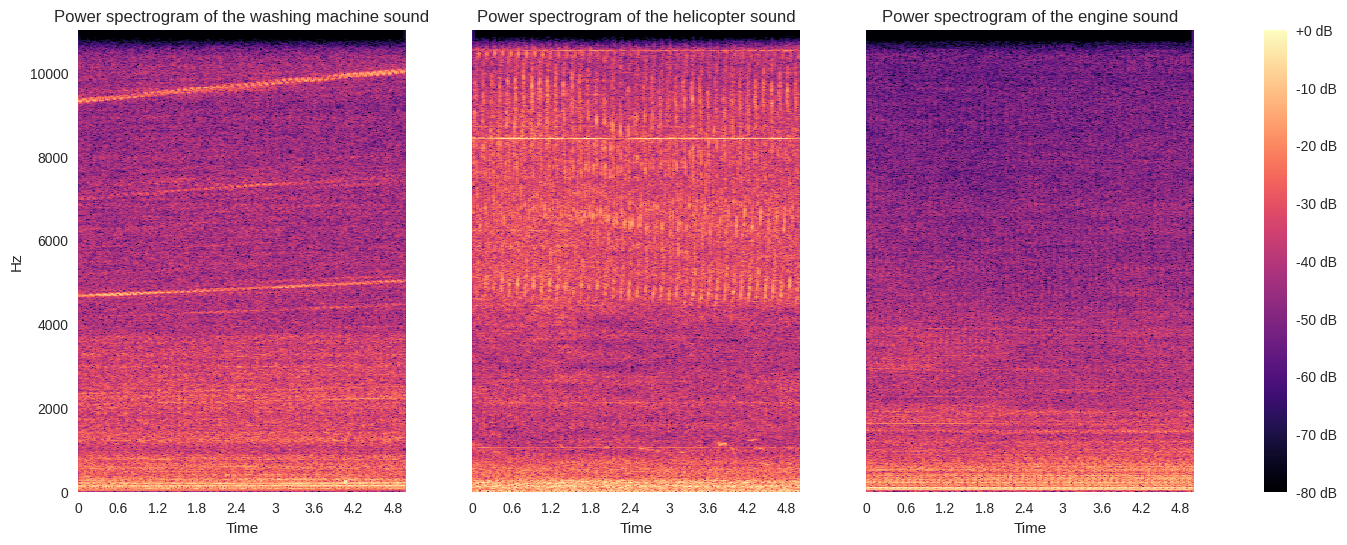
\includegraphics[width=\columnwidth]{Ambiguous_sounds.png}}
  \caption{Power spectrogram of the sound produced by a washing machine, an helicopter and an engine.}
  \label{fig:Ambiguous_sounds}
\end{figure}

This misclassification happens not only for machines, but for humans too. This will be taken into account in the results section, where we will see how the model performs on different classes of sounds.

It is also important to note that, even though we consider the same class, the variability of the sounds is very high, as we can see by comparing the spectrograms of three different
samples of the \textit{dog barking} class. As we can see in Fig.~\ref{fig:Dog_barking}, the three spectrograms are very different from each other. According to the classification defined at the beginngin,
the first one can be considered an impulsive sound, the second one a continuous sound, and the third one an intermittent sound. This means that, given the nature of the sound in this class,
the onset information is not so useful.

\begin{figure}[ht]
  \centering
  \centerline{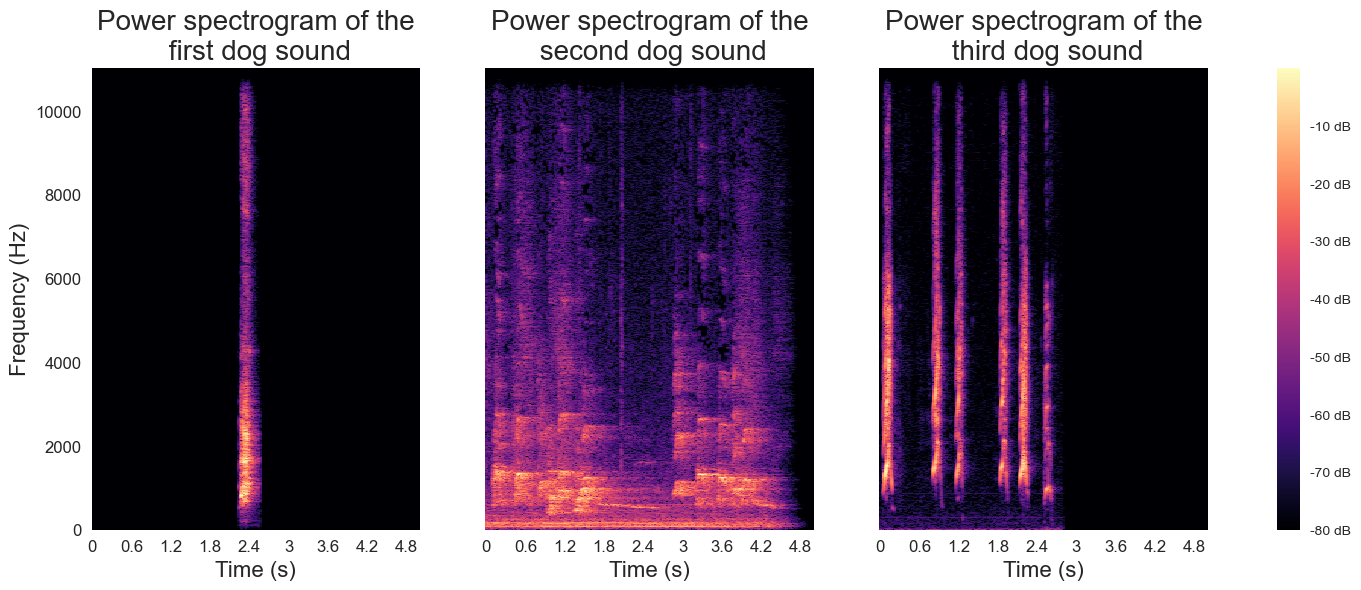
\includegraphics[width=\columnwidth]{dog_barking.png}}
  \caption{Power spectrogram of three different sounds belonging to the same \textit{dog barking} class.}
  \label{fig:Dog_barking}
\end{figure}

Furthermore, we underline how some of the ambiental sounds, like the one of the wind, have no univoque structure: by breaking down their
spectrograms in their harmonic and percussive components as it is done in Fig.~\ref{fig:Dog_barking}, it is evident that the difference
it is not so clear since the two plots are almost equal.

\begin{figure}[ht]
  \centering
  \centerline{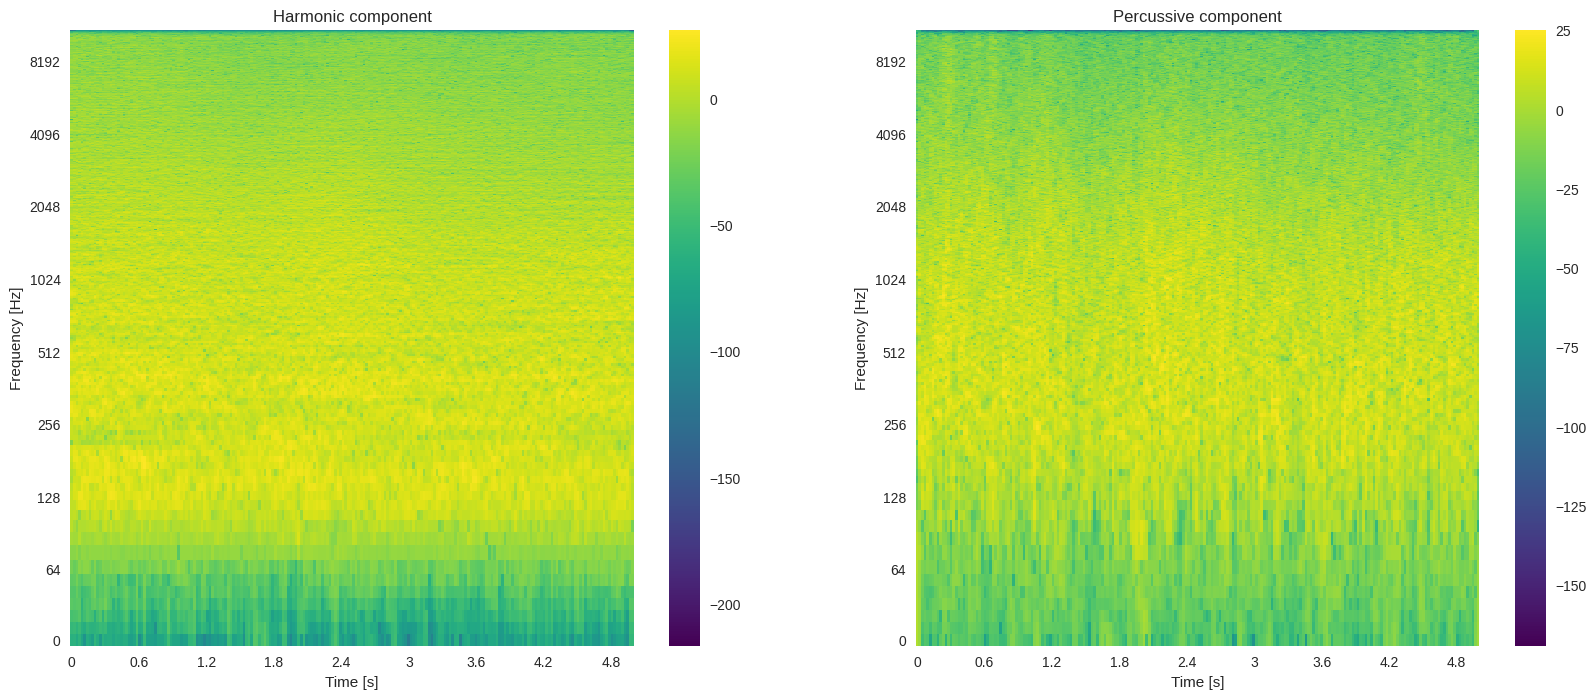
\includegraphics[width=\columnwidth]{Harmonic_Percussive_Wind.png}}
  \caption{Harmonic and percussive decomposition of the wind blowing sound.}
  \label{fig:Harmonic_Percussive_Wind}
\end{figure}

This fast analysis of the dataset has been done to understand the limitations of the model and the difficulties that it could encounter during the training phase.

A part of the dataset, 200 elements (10\% of the total), has been separated for testing. The remaining samples have been splitted according to the stratifiedkfold module of sklearn \cite{scikit-learn_stratifiedkfold} in a training and a validation set.

Drawing inspiration by the Salamon and Bello paper \cite{salamon2017deep}, five different techniques have been implemented to process the training set:
\begin{itemize}
    \item \textbf{Time Stretching (TS)}: the audio signal is stretched or compressed in time by a random factor within a specified range. A last boolean parameter crop the processed audio to the original length, so that the model can be trained on the same length of the original audio.
    \item \textbf{Pitch Shifting (PS)}: the audio signal is shifted in pitch by a random factor within a specified range.
    \item \textbf{Background Noise (BN)}: a Gaussian noise is added to the audio signal with a specified SNR range.
    \item \textbf{Dynamic Range Compression (DRC)}: the dynamic range of the audio signal is compressed from a certain threshold with a specified ratio, attack time, and release time. [Commento: aggiungere che è fatto con la funzione di spotify]
    \item \textbf{Convolution with Impulse Responses (CIR)}: the audio signal is convolved with the \textit{MIT Acoustical Reverberation Scene Statistics Survey} dataset of impulse response \cite{traer2016statistics} to simulate different acoustic environments.
\end{itemize}

For all the results presented in this paper, the training dataset has been preprocessed using the following parameters:
\begin{itemize}
    \item TS: factor between 0.8 and 1.25
    \item PS: factor between -5 and 5 semitones
    \item BN: SNR between 5 and 40 dB
    \item DRC: threshold of -20 dB, ratio of 4:1, attack time of 10 ms, release time of 100 ms
    \item CIR: active
\end{itemize}


\subsection{Evaluation metrics}
\label{sec:metrics}
The evaluation of the sound event classification system is performed using several metrics to assess its performance.
Firstly, the test accuracy, the classification reports and the confusion matrix are computed to evaluate the overall performance of the model.

To evaluate our model, we use 5 folds cross-validation, which allows us to obtain a more robust estimate of the model's performance.
Furthermore, we ensured that there is no data leakage between training and validation sets by doing data augmentation only on the
training set after the splitting.

The training of the models have been performed on the A100 GPU by Google Colab.



\section{Results}
\label{sec:results}
\subsection{Main model results}
\label{sec:main_model_results}
The results of the training of the model for each fold are reported in Figures~\ref{fig:fold0}, \ref{fig:fold1}, \ref{fig:fold2}, \ref{fig:fold3} and \ref{fig:fold4}.
\begin{figure}[ht]
  \centering
  \centerline{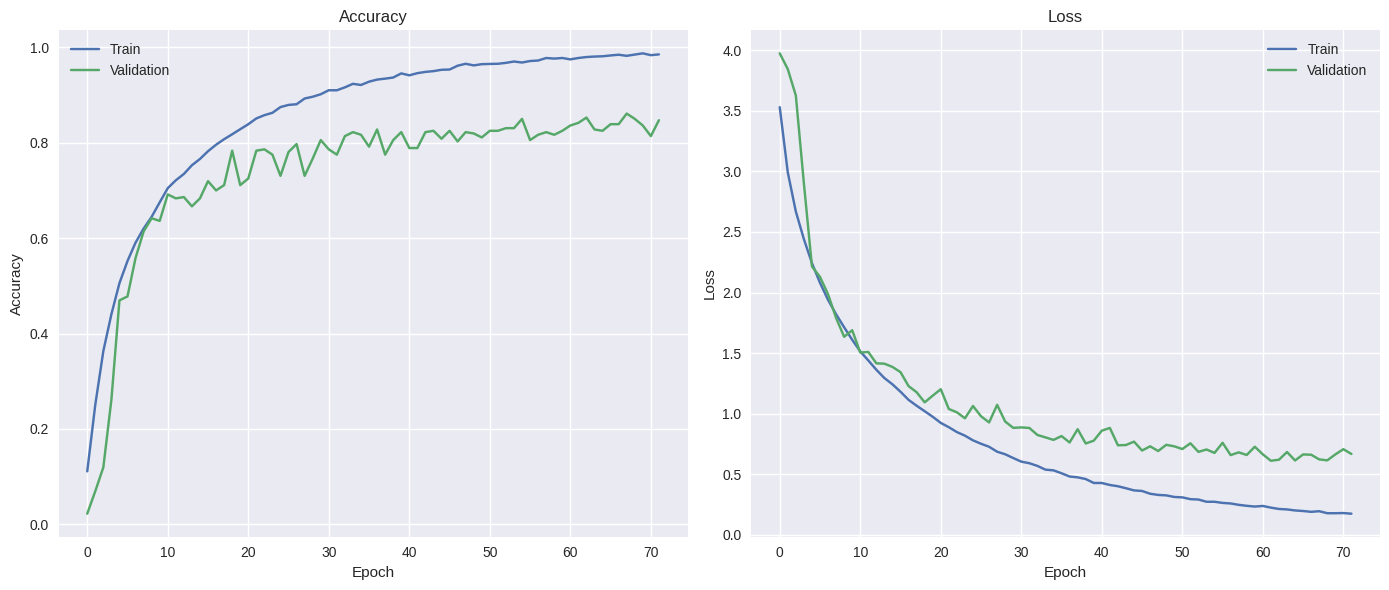
\includegraphics[width=\columnwidth]{fold0.png}}
  \caption{Result of the training for the zero fold.}
  \label{fig:fold0}
\end{figure}

\begin{figure}[ht]
  \centering
  \centerline{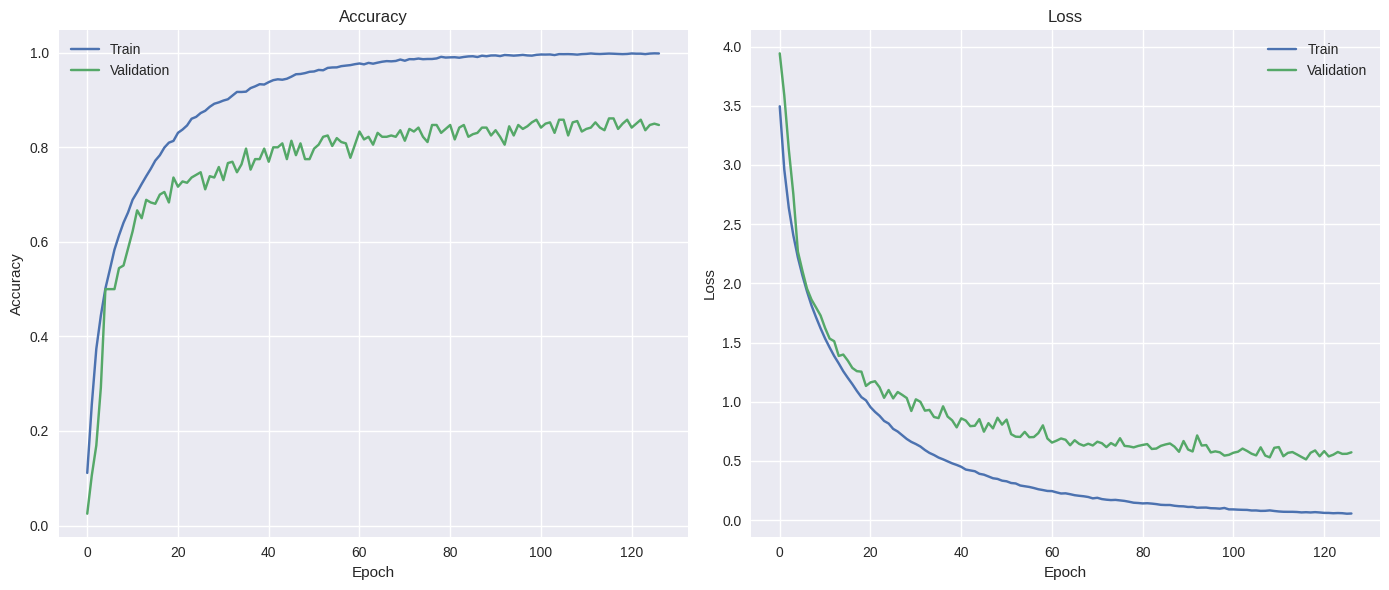
\includegraphics[width=\columnwidth]{fold1.png}}
  \caption{Result of the training for the first fold.}
  \label{fig:fold1}
\end{figure}

\begin{figure}[ht]
  \centering
  \centerline{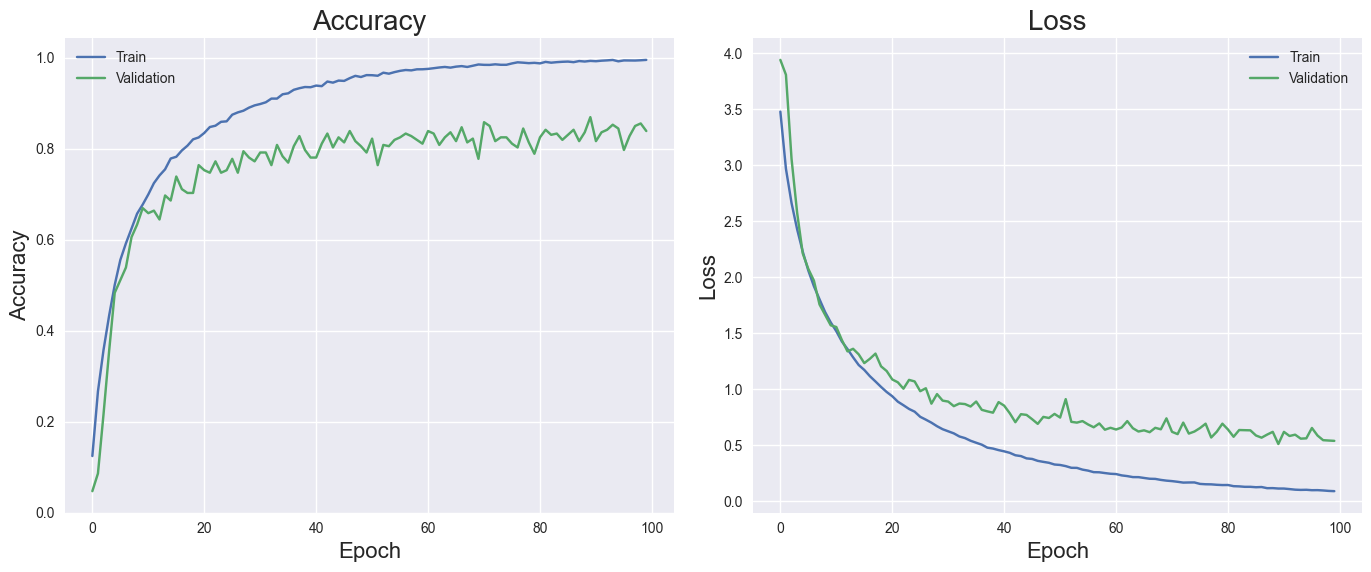
\includegraphics[width=\columnwidth]{fold2.png}}
  \caption{Result of the training for the second fold.}
  \label{fig:fold2}
\end{figure}

\begin{figure}[ht]
  \centering
  \centerline{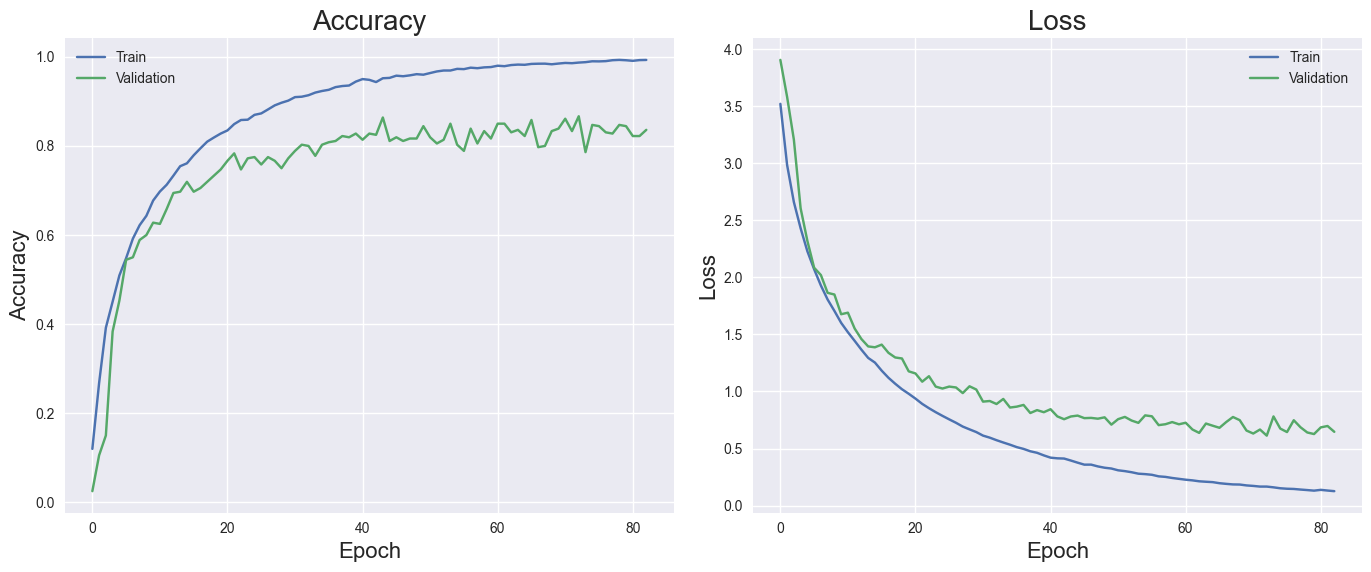
\includegraphics[width=\columnwidth]{fold3.png}}
  \caption{Result of the training for the third fold.}
  \label{fig:fold3}
\end{figure}

\begin{figure}[ht]
  \centering
  \centerline{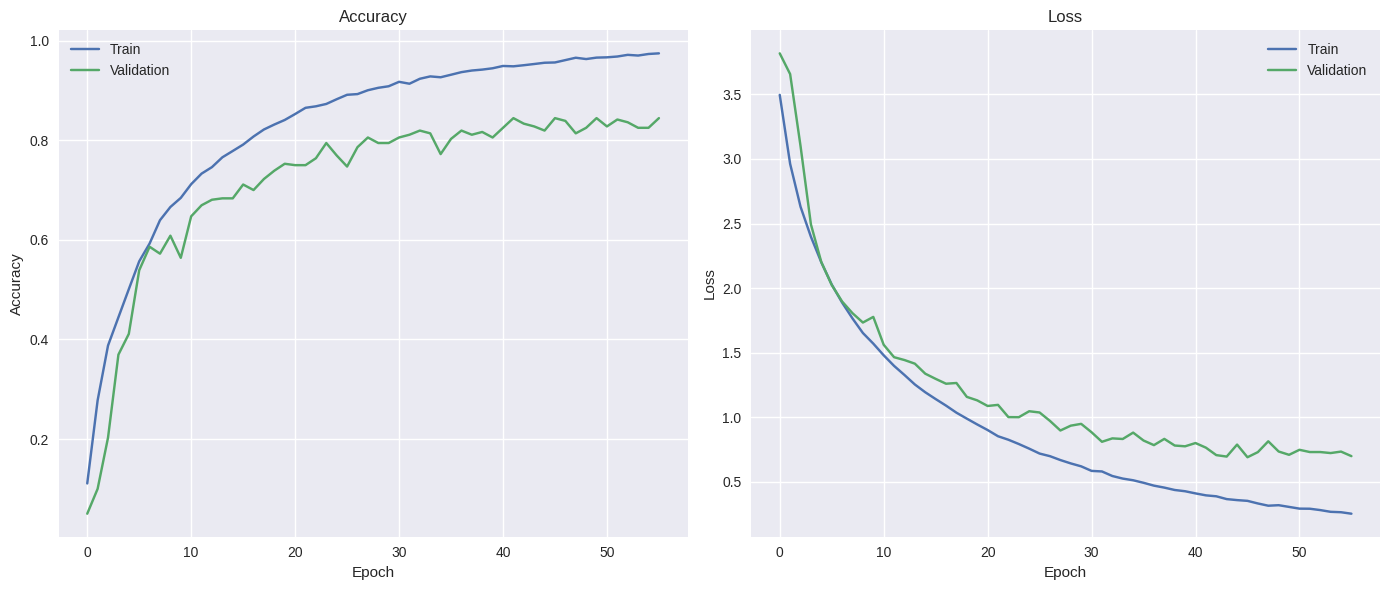
\includegraphics[width=\columnwidth]{fold4.png}}
  \caption{Result of the training for the fourth fold.}
  \label{fig:fold4}
\end{figure}

The average test accuracy over the 5 folds reached by the model is 86\% with an average loss of 0.63.
The performnce for each fold is reported in Table~\ref{tab:folds_results}.

\begin{table}[ht]
  \centering
  \caption{Results of the main model for each fold.}
  \label{tab:folds_results}
  \begin{tabular}{|c|c|c|}
    \hline
    Fold & Test Accuracy & Test Loss \\
    \hline
    0 & 0.85 & 0.65 \\
    1 & 0.87 & 0.60 \\
    2 & 0.88 & 0.58 \\
    3 & 0.86 & 0.62 \\
    4 & 0.85 & 0.64 \\
    \hline
    Average & 0.86 & 0.63 \\
    \hline
    Standard Deviation & 0.024 &  \\
    \hline
  \end{tabular}
\end{table}

In Fig~\ref{fig:confusion_matrix_val} and Fig~\ref{fig:confusion_matrix_test} the
validation and the test confusion matrixes of the model with the best accuracy (88\%) are reported. The
labeling of the classes is reported in the appendix.

\begin{figure}[ht]
  \centering
  \centerline{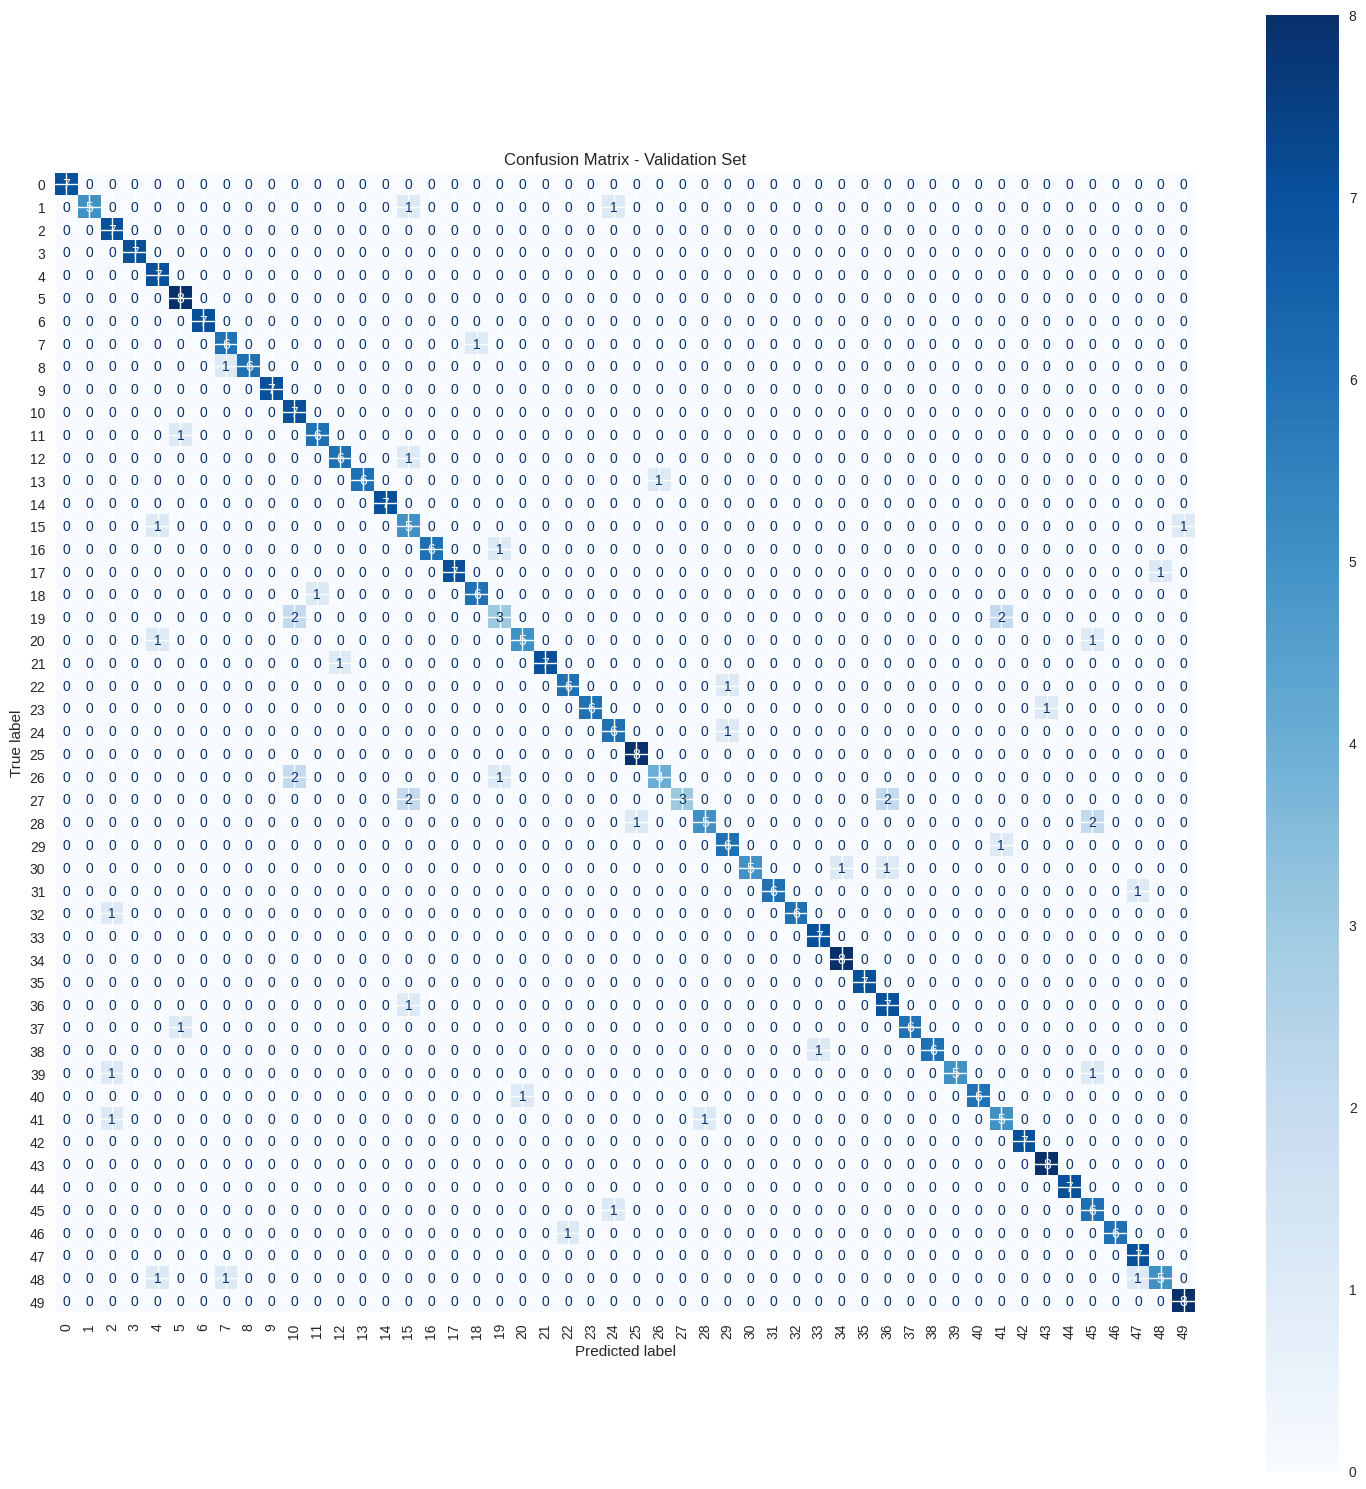
\includegraphics[width=\columnwidth]{Confusion_matrix_val.png}}
  \caption{Confusion Matrix of the validation set.}
  \label{fig:confusion_matrix_val}
\end{figure}

\begin{figure}[ht]
  \centering
  \centerline{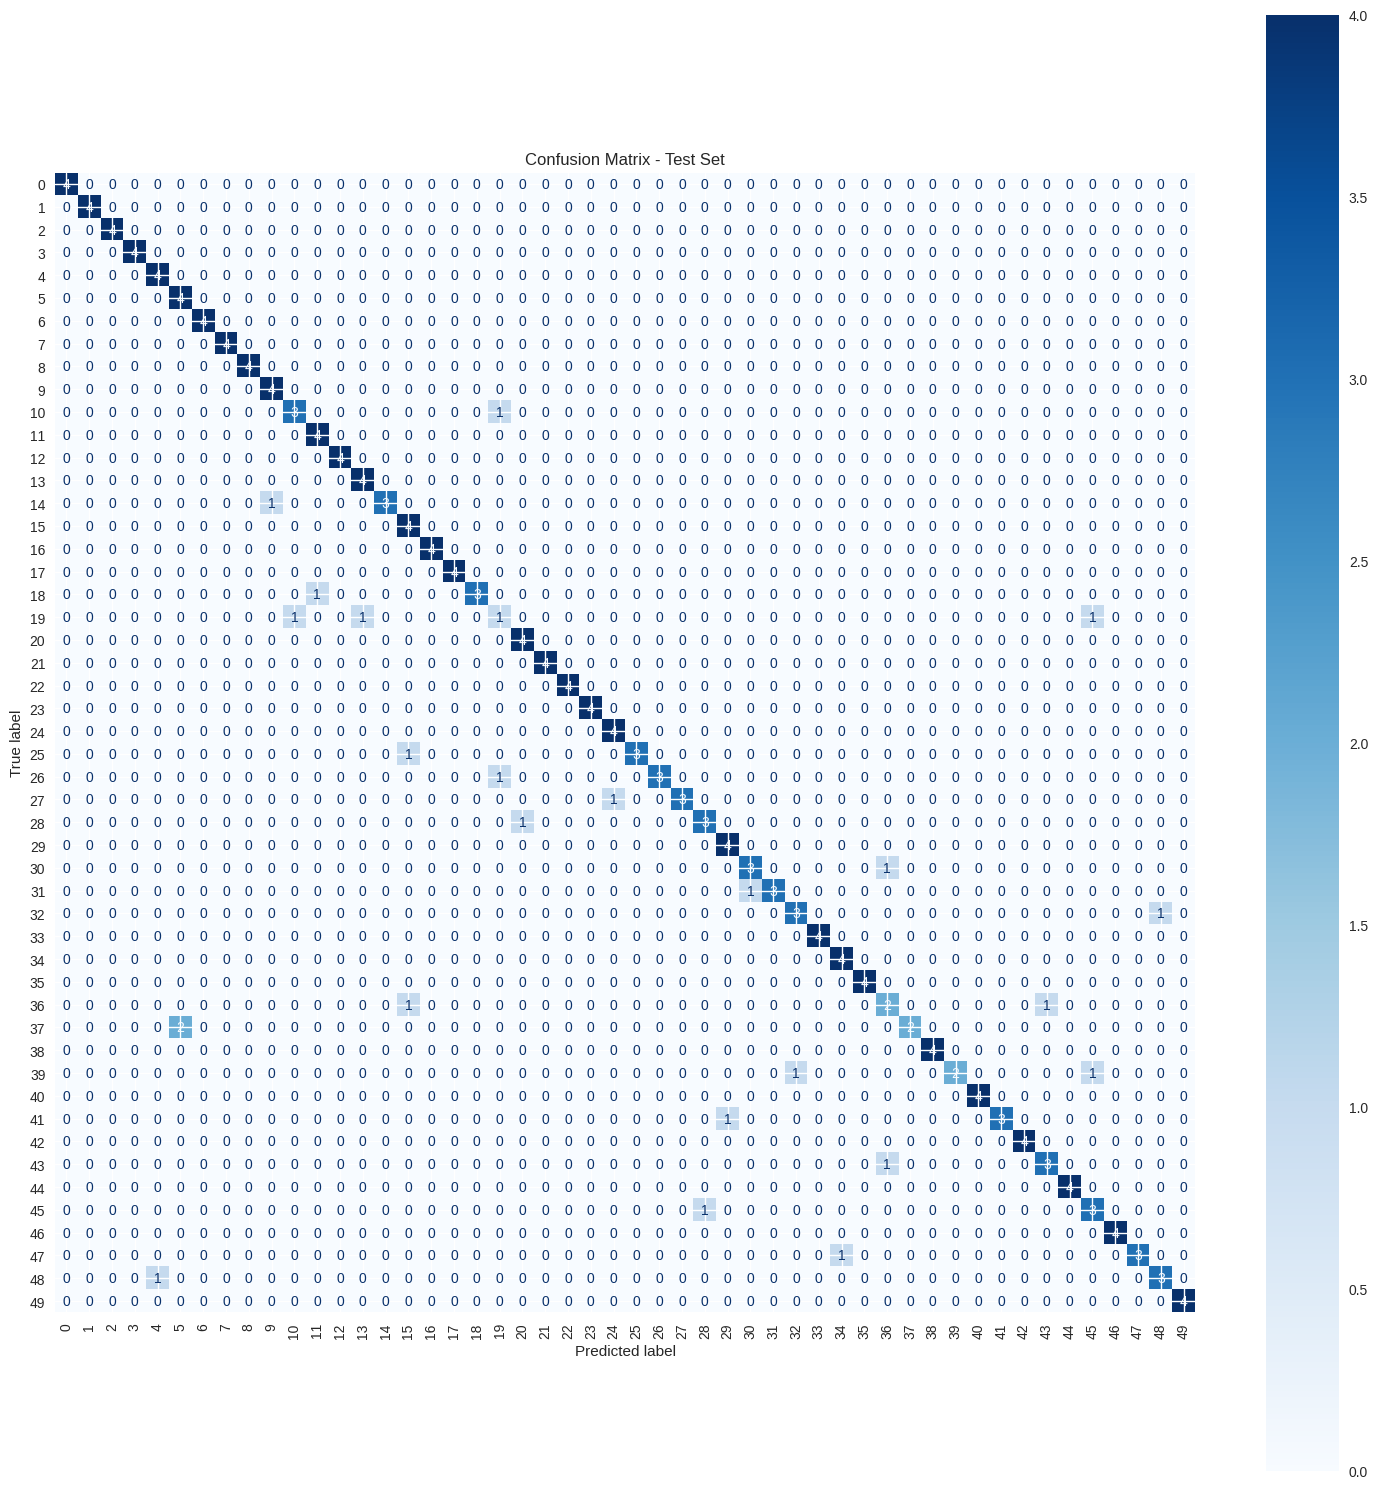
\includegraphics[width=\columnwidth]{Confusion_matrix_test.png}}
  \caption{Confusion Matrix of the test set.}
  \label{fig:confusion_matrix_test}
\end{figure}


The reoprts are reported in Table~\ref{tab:validation_report}
for the validation and in Table~\ref{tab:test_report} for the test.
\begin{table}[ht]
  \centering
  \caption{Classification report on the validation set related to the model with best test accuracy (fold 4).}
  \label{tab:validation_report}
\begin{tabular}{|c|c|c|c|c|}
  \hline
  Class & Precision & Recall & f1-score & Support \\
  \hline
  0  & 1.00 & 1.00 & 1.00 & 7 \\
  1  & 1.00 & 0.71 & 0.83 & 7 \\
  2  & 0.70 & 1.00 & 0.82 & 7 \\
  3  & 1.00 & 1.00 & 1.00 & 7 \\
  4  & 0.70 & 1.00 & 0.82 & 7 \\
  5  & 0.80 & 1.00 & 0.89 & 8 \\
  6  & 1.00 & 1.00 & 1.00 & 7 \\
  7  & 0.75 & 0.86 & 0.80 & 7 \\
  8  & 1.00 & 0.86 & 0.92 & 7 \\
  9  & 1.00 & 1.00 & 1.00 & 7 \\
  10 & 0.64 & 1.00 & 0.78 & 7 \\
  11 & 0.86 & 0.86 & 0.86 & 7 \\
  12 & 0.86 & 0.86 & 0.86 & 7 \\
  13 & 1.00 & 0.86 & 0.92 & 7 \\
  14 & 1.00 & 1.00 & 1.00 & 7 \\
  15 & 0.50 & 0.71 & 0.59 & 7 \\
  16 & 1.00 & 0.86 & 0.92 & 7 \\
  17 & 1.00 & 0.88 & 0.93 & 8 \\
  18 & 0.86 & 0.86 & 0.86 & 7 \\
  19 & 0.60 & 0.43 & 0.50 & 7 \\
  20 & 0.83 & 0.71 & 0.77 & 7 \\
  21 & 1.00 & 0.88 & 0.93 & 8 \\
  22 & 0.86 & 0.86 & 0.86 & 7 \\
  23 & 1.00 & 0.86 & 0.92 & 7 \\
  24 & 0.75 & 0.86 & 0.80 & 7 \\
  25 & 0.89 & 1.00 & 0.94 & 8 \\
  26 & 0.80 & 0.57 & 0.67 & 7 \\
  27 & 1.00 & 0.43 & 0.60 & 7 \\
  28 & 0.83 & 0.62 & 0.71 & 8 \\
  29 & 0.75 & 0.86 & 0.80 & 7 \\
  30 & 1.00 & 0.71 & 0.83 & 7 \\
  31 & 1.00 & 0.86 & 0.92 & 7 \\
  32 & 1.00 & 0.86 & 0.92 & 7 \\
  33 & 0.88 & 1.00 & 0.93 & 7 \\
  34 & 0.89 & 1.00 & 0.94 & 8 \\
  35 & 1.00 & 1.00 & 1.00 & 7 \\
  36 & 0.70 & 0.88 & 0.78 & 8 \\
  37 & 1.00 & 0.86 & 0.92 & 7 \\
  38 & 1.00 & 0.86 & 0.92 & 7 \\
  39 & 1.00 & 0.71 & 0.83 & 7 \\
  40 & 1.00 & 0.86 & 0.92 & 7 \\
  41 & 0.62 & 0.71 & 0.67 & 7 \\
  42 & 1.00 & 1.00 & 1.00 & 7 \\
  43 & 0.89 & 1.00 & 0.94 & 8 \\
  44 & 1.00 & 1.00 & 1.00 & 7 \\
  45 & 0.60 & 0.86 & 0.71 & 7 \\
  46 & 1.00 & 0.86 & 0.92 & 7 \\
  47 & 0.78 & 1.00 & 0.88 & 7 \\
  48 & 0.83 & 0.62 & 0.71 & 8 \\
  49 & 0.89 & 1.00 & 0.94 & 8 \\
  \hline
  Accuracy &  &  & 0.86 & 360 \\
  Marco avg & 0.88 & 0.86 & 0.86 & 360 \\
  Weighted avg & 0.88 & 0.86 & 0.86 & 360 \\
  \hline
  \end{tabular}
\end{table}

\begin{table}[ht]
  \centering
  \caption{Classification report on the test set related to the model with best test accuracy (fold 4).}
  \label{tab:test_report}
  \begin{tabular}{|c|c|c|c|c|}
  \hline
  Class & Precision & Recall & f1-score & Support \\
  \hline
  0  & 1.00 & 1.00 & 1.00 & 4 \\
  1  & 1.00 & 1.00 & 1.00 & 4 \\
  2  & 1.00 & 1.00 & 1.00 & 4 \\
  3  & 1.00 & 1.00 & 1.00 & 4 \\
  4  & 0.80 & 1.00 & 0.89 & 4 \\
  5  & 0.67 & 1.00 & 0.80 & 4 \\
  6  & 1.00 & 1.00 & 1.00 & 4 \\
  7  & 1.00 & 1.00 & 1.00 & 4 \\
  8  & 1.00 & 1.00 & 1.00 & 4 \\
  9  & 0.80 & 1.00 & 0.89 & 4 \\
  10 & 0.75 & 0.75 & 0.75 & 4 \\
  11 & 0.80 & 1.00 & 0.89 & 4 \\
  12 & 1.00 & 1.00 & 1.00 & 4 \\
  13 & 0.80 & 1.00 & 0.89 & 4 \\
  14 & 1.00 & 0.75 & 0.86 & 4 \\
  15 & 0.67 & 1.00 & 0.80 & 4 \\
  16 & 1.00 & 1.00 & 1.00 & 4 \\
  17 & 1.00 & 1.00 & 1.00 & 4 \\
  18 & 1.00 & 0.75 & 0.86 & 4 \\
  19 & 0.33 & 0.25 & 0.29 & 4 \\
  20 & 0.80 & 1.00 & 0.89 & 4 \\
  21 & 1.00 & 1.00 & 1.00 & 4 \\
  22 & 1.00 & 1.00 & 1.00 & 4 \\
  23 & 1.00 & 1.00 & 1.00 & 4 \\
  24 & 0.80 & 1.00 & 0.89 & 4 \\
  25 & 1.00 & 0.75 & 0.86 & 4 \\
  26 & 1.00 & 0.75 & 0.86 & 4 \\
  27 & 1.00 & 0.75 & 0.86 & 4 \\
  28 & 0.75 & 0.75 & 0.75 & 4 \\
  29 & 0.80 & 1.00 & 0.89 & 4 \\
  30 & 0.75 & 0.75 & 0.75 & 4 \\
  31 & 1.00 & 0.75 & 0.86 & 4 \\
  32 & 0.75 & 0.75 & 0.75 & 4 \\
  33 & 1.00 & 1.00 & 1.00 & 4 \\
  34 & 0.80 & 1.00 & 0.89 & 4 \\
  35 & 1.00 & 1.00 & 1.00 & 4 \\
  36 & 0.50 & 0.50 & 0.50 & 4 \\
  37 & 1.00 & 0.50 & 0.67 & 4 \\
  38 & 1.00 & 1.00 & 1.00 & 4 \\
  39 & 1.00 & 0.50 & 0.67 & 4 \\
  40 & 1.00 & 1.00 & 1.00 & 4 \\
  41 & 1.00 & 0.75 & 0.86 & 4 \\
  42 & 1.00 & 1.00 & 1.00 & 4 \\
  43 & 0.75 & 0.75 & 0.75 & 4 \\
  44 & 1.00 & 1.00 & 1.00 & 4 \\
  45 & 0.60 & 0.75 & 0.67 & 4 \\
  46 & 1.00 & 1.00 & 1.00 & 4 \\
  47 & 1.00 & 0.75 & 0.86 & 4 \\
  48 & 0.75 & 0.75 & 0.75 & 4 \\
  49 & 1.00 & 1.00 & 1.00 & 4 \\
  \hline
  Accuracy & & & 0.88 & 200 \\
  Macro avg & 0.89 & 0.88 & 0.88 & 200 \\
  Weighted avg & 0.89 & 0.88 & 0.88 & 200 \\
  \hline
  \end{tabular}
\end{table}

We highlight here how precision and recall are well balanced meaning that the model is not biased towards a specific class.
\newline
By looking at the test confusion matrix, we can see that the model is able to classify correctly most of the sounds, with some exceptions.
One of them is the \textit{wind} class that is misclassified 3 times out of 4: one time classified as
\textit{train}, one as \textit{airplane} and as \textit{sea waves}. As we can notice, all the three sounds
are continuous and noisy sounds, so it is not surprising that the model has some difficulties in classifying them.
This match with what we assumed by looking at Fig.~\ref{fig:Ambiguous_sounds}: sounds with similar spectrograms are
more difficult to classify. It is interesting to notice that the recall of these three classes is not high even in the 
results of the experiment conducted by Piczak \cite{piczak2015dataset} in which a group oh humnas listened to the sounds and classified them.
This leads us to think that since the model is inspired by the human auditory system, it is not surprising that it has the same difficulties in classifying the sounds. 

Another class that is misclassified is the \textit{coughing} class, which is confused with the 
\textit{sneezing} and \textit{water drops} class. We underline how all these sounds are intermittent sounds
and that they have similar spectrograms.

For what it concerns false positive, these are the errors made by the model: the sound of the \textit{airplane} and
\textit{helicopter} has been classified as \textit{wind}, the sound of \textit{sneezing} and \textit{laughing} as \textit{caughing}
and for two times the \textit{glass breaking} sound has been misclassified as \textit{can opening}. We can justify
these results by claiming the same motivation we exposed before: similar spectrograms lead to misclassification.

[Commento: manca il confronto con la baseline]

\subsection{Comparison: main model with different inputs}
\label{sec:comparison_1}
During the training of the main model, we tried to use different inputs to see how they affect the performance of the model.
At the end, we notice that all the results are similar, with a slight improvement in the accuracy when using the log mel-spectrogram as input.
They are reported in Table~\ref{tab:comparison_inputs}.
\begin{table}[ht]
  \centering
  \caption{Performances for different inputs.}
  \label{tab:comparison_inputs}
  \begin{tabular}{|c|c|c|}
    \hline
    Input & Test Accuracy & Test Loss \\
    \hline
    log mel-spectrogram & 0.86 & 0.63 \\
    log STFT & 0.83 & 0.71 \\
    MFCCs & 0.78 & 0.78 \\
    \hline
  \end{tabular}
\end{table}

We notice how MFCCs are the worst input. This could seems strange thinking that MFFCs are the most processed input we can use among the ones tested.
MFCCs could be effective with classical machine learning algorithms, where the features were extracted from the raw data and then used to train the model.
However, with the improvements made by neural networks, is no longer necessary perform classical feature engineering since the networks
are able to extract better features by themselves. For what we just said, we can undesrtand why even the simple
STFT works better than MFCCs.

\subsection{Comparison: main model with }
\label{sec:comparison_2}

\section{Acknowledgments}
\label{sec:ack}


This work was supported by the Politecnico di Milano,
within the framework of the Selected Topics in Music and Acoustic Engineering Course 2025.
A special thanks goes to the course instructor, Prof. JULIO JOSÉ CARABIAS ORTI, for being
one of the brightest stars in the sky of artificial intelligence.
Last but not least, we would like to thank our wallet: without those 24 euros, we would not have been able to run anything.
Thank you for your support, we are grateful for your generosity.
Grazie a tutt coloro che ci hanno supportato e sopportato.
% -------------------------------------------------------------------------
% Either list references using the bibliography style file IEEEtran.bst
\bibliographystyle{IEEEtran}
\bibliography{refs21}
\section{Appendix - Sound classes}
\label{sec:Appendix}
\begin{itemize}
  \item 0: dog
  \item 1: chirping birds
  \item 2: vacuum cleaner
  \item 3: thunderstorm
  \item 4: door wood knock
  \item 5: can opening
  \item 6: crow
  \item 7: clapping
  \item 8: fireworks
  \item 9: chainsaw
  \item 10: airplane
  \item 11: mouse click
  \item 12: pouring water
  \item 13: train
  \item 14: sheep
  \item 15: water drops
  \item 16: church bells
  \item 17: clock alarm
  \item 18: keyboard typing
  \item 19: wind
  \item 20: footsteps
  \item 21: frog
  \item 22: cow
  \item 23: brushing teeth
  \item 24: car horn
  \item 25: crackling fire
  \item 26: helicopter
  \item 27: drinking sipping
  \item 28: rain
  \item 29: insects
  \item 30: laughing
  \item 31: hen
  \item 32: engine
  \item 33: breathing
  \item 34: crying baby
  \item 35: hand saw
  \item 36: coughing
  \item 37: glass breaking
  \item 38: snoring
  \item 39: toilet flush
  \item 40: pig
  \item 41: washing machine
  \item 42: clock tick
  \item 43: sneezing
  \item 44: rooster
  \item 45: sea waves
  \item 46: siren
  \item 47: cat
  \item 48: door wood creaks
  \item 49: crickets
\end{itemize}

\end{sloppy}
\end{document}
